\documentclass[twoside]{book}

% Packages required by doxygen
\usepackage{fixltx2e}
\usepackage{calc}
\usepackage{doxygen}
\usepackage[export]{adjustbox} % also loads graphicx
\usepackage{graphicx}
\usepackage[utf8]{inputenc}
\usepackage{makeidx}
\usepackage{multicol}
\usepackage{multirow}
\PassOptionsToPackage{warn}{textcomp}
\usepackage{textcomp}
\usepackage[nointegrals]{wasysym}
\usepackage[table]{xcolor}

% Font selection
\usepackage[T1]{fontenc}
\usepackage[scaled=.90]{helvet}
\usepackage{courier}
\usepackage{amssymb}
\usepackage{sectsty}
\renewcommand{\familydefault}{\sfdefault}
\allsectionsfont{%
  \fontseries{bc}\selectfont%
  \color{darkgray}%
}
\renewcommand{\DoxyLabelFont}{%
  \fontseries{bc}\selectfont%
  \color{darkgray}%
}
\newcommand{\+}{\discretionary{\mbox{\scriptsize$\hookleftarrow$}}{}{}}

% Page & text layout
\usepackage{geometry}
\geometry{%
  a4paper,%
  top=2.5cm,%
  bottom=2.5cm,%
  left=2.5cm,%
  right=2.5cm%
}
\tolerance=750
\hfuzz=15pt
\hbadness=750
\setlength{\emergencystretch}{15pt}
\setlength{\parindent}{0cm}
\setlength{\parskip}{3ex plus 2ex minus 2ex}
\makeatletter
\renewcommand{\paragraph}{%
  \@startsection{paragraph}{4}{0ex}{-1.0ex}{1.0ex}{%
    \normalfont\normalsize\bfseries\SS@parafont%
  }%
}
\renewcommand{\subparagraph}{%
  \@startsection{subparagraph}{5}{0ex}{-1.0ex}{1.0ex}{%
    \normalfont\normalsize\bfseries\SS@subparafont%
  }%
}
\makeatother

% Headers & footers
\usepackage{fancyhdr}
\pagestyle{fancyplain}
\fancyhead[LE]{\fancyplain{}{\bfseries\thepage}}
\fancyhead[CE]{\fancyplain{}{}}
\fancyhead[RE]{\fancyplain{}{\bfseries\leftmark}}
\fancyhead[LO]{\fancyplain{}{\bfseries\rightmark}}
\fancyhead[CO]{\fancyplain{}{}}
\fancyhead[RO]{\fancyplain{}{\bfseries\thepage}}
\fancyfoot[LE]{\fancyplain{}{}}
\fancyfoot[CE]{\fancyplain{}{}}
\fancyfoot[RE]{\fancyplain{}{\bfseries\scriptsize Generated by Doxygen }}
\fancyfoot[LO]{\fancyplain{}{\bfseries\scriptsize Generated by Doxygen }}
\fancyfoot[CO]{\fancyplain{}{}}
\fancyfoot[RO]{\fancyplain{}{}}
\renewcommand{\footrulewidth}{0.4pt}
\renewcommand{\chaptermark}[1]{%
  \markboth{#1}{}%
}
\renewcommand{\sectionmark}[1]{%
  \markright{\thesection\ #1}%
}

% Indices & bibliography
\usepackage{natbib}
\usepackage[titles]{tocloft}
\setcounter{tocdepth}{3}
\setcounter{secnumdepth}{5}
\makeindex

% Hyperlinks (required, but should be loaded last)
\usepackage{ifpdf}
\ifpdf
  \usepackage[pdftex,pagebackref=true]{hyperref}
\else
  \usepackage[ps2pdf,pagebackref=true]{hyperref}
\fi
\hypersetup{%
  colorlinks=true,%
  linkcolor=blue,%
  citecolor=blue,%
  unicode%
}

% Custom commands
\newcommand{\clearemptydoublepage}{%
  \newpage{\pagestyle{empty}\cleardoublepage}%
}

\usepackage{caption}
\captionsetup{labelsep=space,justification=centering,font={bf},singlelinecheck=off,skip=4pt,position=top}

%===== C O N T E N T S =====

\begin{document}

% Titlepage & ToC
\hypersetup{pageanchor=false,
             bookmarksnumbered=true,
             pdfencoding=unicode
            }
\pagenumbering{alph}
\begin{titlepage}
\vspace*{7cm}
\begin{center}%
{\Large pclregister }\\
\vspace*{1cm}
{\large Generated by Doxygen 1.8.12}\\
\end{center}
\end{titlepage}
\clearemptydoublepage
\pagenumbering{roman}
\tableofcontents
\clearemptydoublepage
\pagenumbering{arabic}
\hypersetup{pageanchor=true}

%--- Begin generated contents ---
\chapter{Class Index}
\section{Class List}
Here are the classes, structs, unions and interfaces with brief descriptions\+:\begin{DoxyCompactList}
\item\contentsline{section}{\hyperlink{class_features}{Features} }{\pageref{class_features}}{}
\item\contentsline{section}{\hyperlink{class_filters}{Filters} }{\pageref{class_filters}}{}
\item\contentsline{section}{\hyperlink{class_loader}{Loader} }{\pageref{class_loader}}{}
\item\contentsline{section}{\hyperlink{struct_features_1_1_object_features}{Features\+::\+Object\+Features} }{\pageref{struct_features_1_1_object_features}}{}
\item\contentsline{section}{\hyperlink{class_registrator}{Registrator} }{\pageref{class_registrator}}{}
\item\contentsline{section}{\hyperlink{class_saver}{Saver} }{\pageref{class_saver}}{}
\end{DoxyCompactList}

\chapter{File Index}
\section{File List}
Here is a list of all files with brief descriptions\+:\begin{DoxyCompactList}
\item\contentsline{section}{include/\hyperlink{features_8hpp}{features.\+hpp} }{\pageref{features_8hpp}}{}
\item\contentsline{section}{include/\hyperlink{filters_8hpp}{filters.\+hpp} }{\pageref{filters_8hpp}}{}
\item\contentsline{section}{include/\hyperlink{loader_8hpp}{loader.\+hpp} }{\pageref{loader_8hpp}}{}
\item\contentsline{section}{include/\hyperlink{registrator_8hpp}{registrator.\+hpp} }{\pageref{registrator_8hpp}}{}
\item\contentsline{section}{src/\hyperlink{features_8cpp}{features.\+cpp} }{\pageref{features_8cpp}}{}
\item\contentsline{section}{src/\hyperlink{filters_8cpp}{filters.\+cpp} }{\pageref{filters_8cpp}}{}
\item\contentsline{section}{src/\hyperlink{loader_8cpp}{loader.\+cpp} }{\pageref{loader_8cpp}}{}
\item\contentsline{section}{src/\hyperlink{main_8cpp}{main.\+cpp} }{\pageref{main_8cpp}}{}
\item\contentsline{section}{src/\hyperlink{registrator_8cpp}{registrator.\+cpp} }{\pageref{registrator_8cpp}}{}
\end{DoxyCompactList}

\chapter{Class Documentation}
\hypertarget{class_features}{}\section{Features Class Reference}
\label{class_features}\index{Features@{Features}}


{\ttfamily \#include $<$features.\+hpp$>$}

\subsection*{Classes}
\begin{DoxyCompactItemize}
\item 
struct \hyperlink{struct_features_1_1_object_features}{Object\+Features}
\end{DoxyCompactItemize}
\subsection*{Public Member Functions}
\begin{DoxyCompactItemize}
\item 
pcl\+::\+Point\+Cloud$<$ pcl\+::\+Normal $>$\+::Ptr \hyperlink{class_features_a925cf73afb0607d0fe74a47347ec670d}{estimate\+Surface\+Normals} (const pcl\+::\+Point\+Cloud$<$ pcl\+::\+Point\+X\+Y\+Z\+R\+GB $>$\+::Ptr \&input\+Cloud, float radius)
\item 
pcl\+::\+Point\+Cloud$<$ pcl\+::\+Point\+X\+Y\+Z\+R\+GB $>$\+::Ptr \hyperlink{class_features_a5c6f5430e675a9216da80875e700f32e}{detect\+Keypoints} (const pcl\+::\+Point\+Cloud$<$ pcl\+::\+Point\+X\+Y\+Z\+R\+GB $>$\+::Ptr \&points, const pcl\+::\+Point\+Cloud$<$ pcl\+::\+Normal $>$\+::Ptr \&normals, float min\+\_\+scale, int nr\+\_\+octaves, int nr\+\_\+scales\+\_\+per\+\_\+octave, float min\+\_\+contrast)
\item 
pcl\+::\+Point\+Cloud$<$ pcl\+::\+F\+P\+F\+H\+Signature33 $>$\+::Ptr \hyperlink{class_features_a9a35a8508f21553be97a868a167ac2de}{compute\+Local\+Descriptors} (const pcl\+::\+Point\+Cloud$<$ pcl\+::\+Point\+X\+Y\+Z\+R\+GB $>$\+::Ptr \&points, const pcl\+::\+Point\+Cloud$<$ pcl\+::\+Normal $>$\+::Ptr \&normals, const pcl\+::\+Point\+Cloud$<$ pcl\+::\+Point\+X\+Y\+Z\+R\+GB $>$\+::Ptr \&keypoints, float feature\+\_\+radius)
\item 
pcl\+::\+Point\+Cloud$<$ pcl\+::\+V\+F\+H\+Signature308 $>$\+::Ptr \hyperlink{class_features_a6e7efba994adbfa03682e796ed932a99}{compute\+Global\+Descriptor} (const pcl\+::\+Point\+Cloud$<$ pcl\+::\+Point\+X\+Y\+Z\+R\+GB $>$\+::Ptr \&points, const pcl\+::\+Point\+Cloud$<$ pcl\+::\+Normal $>$\+::Ptr \&normals)
\item 
boost\+::shared\+\_\+ptr$<$ \hyperlink{struct_features_1_1_object_features}{Features\+::\+Object\+Features} $>$ \hyperlink{class_features_ad1d4524155b37393ae8b64f0c5c0d553}{compute\+Features} (const pcl\+::\+Point\+Cloud$<$ pcl\+::\+Point\+X\+Y\+Z\+R\+GB $>$\+::Ptr \&input)
\end{DoxyCompactItemize}


\subsection{Detailed Description}
This class is used solely for feature detection of various point clouds (e.\+g. interest points) 

Definition at line 11 of file features.\+hpp.



\subsection{Member Function Documentation}
\hypertarget{class_features_ad1d4524155b37393ae8b64f0c5c0d553}{}\label{class_features_ad1d4524155b37393ae8b64f0c5c0d553} 
\index{Features@{Features}!compute\+Features@{compute\+Features}}
\index{compute\+Features@{compute\+Features}!Features@{Features}}
\subsubsection{\texorpdfstring{compute\+Features()}{computeFeatures()}}
{\footnotesize\ttfamily boost\+::shared\+\_\+ptr$<$ \hyperlink{struct_features_1_1_object_features}{Features\+::\+Object\+Features} $>$ Features\+::compute\+Features (\begin{DoxyParamCaption}\item[{const pcl\+::\+Point\+Cloud$<$ pcl\+::\+Point\+X\+Y\+Z\+R\+GB $>$\+::Ptr \&}]{input }\end{DoxyParamCaption})}

Estimate normals, detect keypoints, and compute local and global descriptors Return\+: An \hyperlink{struct_features_1_1_object_features}{Object\+Features} struct containing all the features 

Definition at line 133 of file features.\+cpp.

Here is the call graph for this function\+:
\nopagebreak
\begin{figure}[H]
\begin{center}
\leavevmode
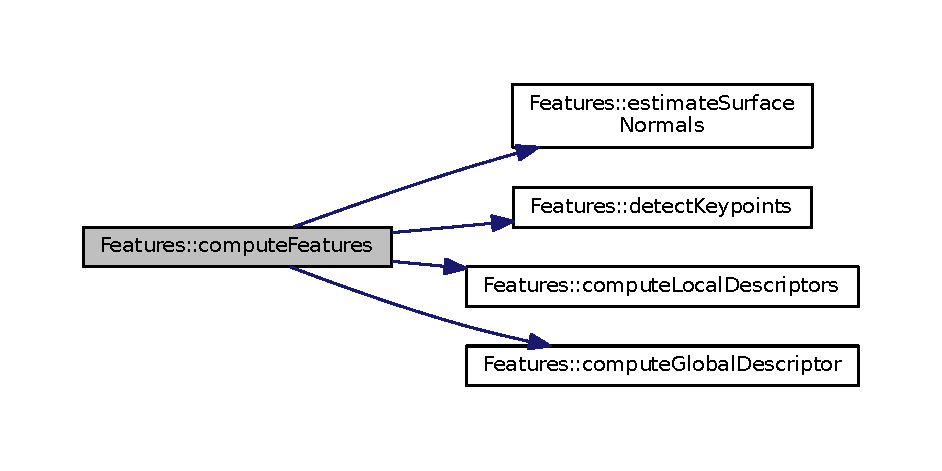
\includegraphics[width=350pt]{class_features_ad1d4524155b37393ae8b64f0c5c0d553_cgraph}
\end{center}
\end{figure}
\hypertarget{class_features_a6e7efba994adbfa03682e796ed932a99}{}\label{class_features_a6e7efba994adbfa03682e796ed932a99} 
\index{Features@{Features}!compute\+Global\+Descriptor@{compute\+Global\+Descriptor}}
\index{compute\+Global\+Descriptor@{compute\+Global\+Descriptor}!Features@{Features}}
\subsubsection{\texorpdfstring{compute\+Global\+Descriptor()}{computeGlobalDescriptor()}}
{\footnotesize\ttfamily pcl\+::\+Point\+Cloud$<$ pcl\+::\+V\+F\+H\+Signature308 $>$\+::Ptr Features\+::compute\+Global\+Descriptor (\begin{DoxyParamCaption}\item[{const pcl\+::\+Point\+Cloud$<$ pcl\+::\+Point\+X\+Y\+Z\+R\+GB $>$\+::Ptr \&}]{points,  }\item[{const pcl\+::\+Point\+Cloud$<$ pcl\+::\+Normal $>$\+::Ptr \&}]{normals }\end{DoxyParamCaption})}

Use V\+F\+H\+Estimation to compute a single global descriptor for the entire input cloud Inputs\+: points The input point cloud normals The input surface normals Return\+: A pointer to a Global\+Descriptors point cloud (a cloud containing a single Global\+DescriptorT point) 

Definition at line 108 of file features.\+cpp.

Here is the caller graph for this function\+:
\nopagebreak
\begin{figure}[H]
\begin{center}
\leavevmode
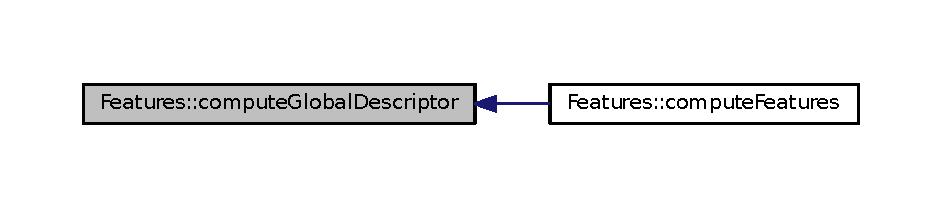
\includegraphics[width=350pt]{class_features_a6e7efba994adbfa03682e796ed932a99_icgraph}
\end{center}
\end{figure}
\hypertarget{class_features_a9a35a8508f21553be97a868a167ac2de}{}\label{class_features_a9a35a8508f21553be97a868a167ac2de} 
\index{Features@{Features}!compute\+Local\+Descriptors@{compute\+Local\+Descriptors}}
\index{compute\+Local\+Descriptors@{compute\+Local\+Descriptors}!Features@{Features}}
\subsubsection{\texorpdfstring{compute\+Local\+Descriptors()}{computeLocalDescriptors()}}
{\footnotesize\ttfamily pcl\+::\+Point\+Cloud$<$ pcl\+::\+F\+P\+F\+H\+Signature33 $>$\+::Ptr Features\+::compute\+Local\+Descriptors (\begin{DoxyParamCaption}\item[{const pcl\+::\+Point\+Cloud$<$ pcl\+::\+Point\+X\+Y\+Z\+R\+GB $>$\+::Ptr \&}]{points,  }\item[{const pcl\+::\+Point\+Cloud$<$ pcl\+::\+Normal $>$\+::Ptr \&}]{normals,  }\item[{const pcl\+::\+Point\+Cloud$<$ pcl\+::\+Point\+X\+Y\+Z\+R\+GB $>$\+::Ptr \&}]{keypoints,  }\item[{float}]{feature\+\_\+radius }\end{DoxyParamCaption})}

Use F\+P\+F\+H\+Estimation to compute local feature descriptors around each keypoint Inputs\+: points The input point cloud normals The input surface normals keypoints A cloud of keypoints specifying the positions at which the descriptors should be computed feature\+\_\+radius The size of the neighborhood from which the local descriptors will be computed Return\+: A pointer to a Local\+Descriptors (a cloud of Local\+DescriptorT points) 

Definition at line 77 of file features.\+cpp.

Here is the caller graph for this function\+:
\nopagebreak
\begin{figure}[H]
\begin{center}
\leavevmode
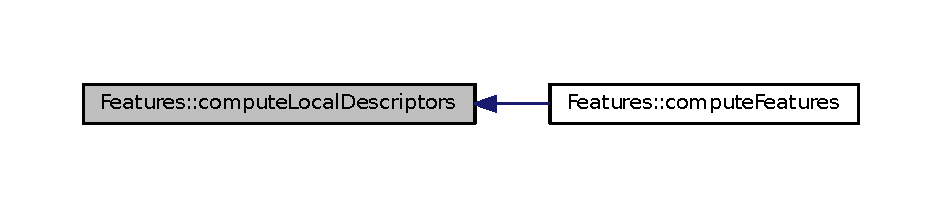
\includegraphics[width=350pt]{class_features_a9a35a8508f21553be97a868a167ac2de_icgraph}
\end{center}
\end{figure}
\hypertarget{class_features_a5c6f5430e675a9216da80875e700f32e}{}\label{class_features_a5c6f5430e675a9216da80875e700f32e} 
\index{Features@{Features}!detect\+Keypoints@{detect\+Keypoints}}
\index{detect\+Keypoints@{detect\+Keypoints}!Features@{Features}}
\subsubsection{\texorpdfstring{detect\+Keypoints()}{detectKeypoints()}}
{\footnotesize\ttfamily pcl\+::\+Point\+Cloud$<$ pcl\+::\+Point\+X\+Y\+Z\+R\+GB $>$\+::Ptr Features\+::detect\+Keypoints (\begin{DoxyParamCaption}\item[{const pcl\+::\+Point\+Cloud$<$ pcl\+::\+Point\+X\+Y\+Z\+R\+GB $>$\+::Ptr \&}]{points,  }\item[{const pcl\+::\+Point\+Cloud$<$ pcl\+::\+Normal $>$\+::Ptr \&}]{normals,  }\item[{float}]{min\+\_\+scale,  }\item[{int}]{nr\+\_\+octaves,  }\item[{int}]{nr\+\_\+scales\+\_\+per\+\_\+octave,  }\item[{float}]{min\+\_\+contrast }\end{DoxyParamCaption})}

Use S\+I\+F\+T\+Keypoint to detect a set of keypoints Inputs\+: points The input point cloud normals The input surface normals min\+\_\+scale The smallest scale in the difference-\/of-\/\+Gaussians (DoG) scale-\/space nr\+\_\+octaves The number of times the scale doubles in the DoG scale-\/space nr\+\_\+scales\+\_\+per\+\_\+octave The number of scales computed for each doubling min\+\_\+contrast The minimum local contrast that must be present for a keypoint to be detected Return\+: A pointer to a point cloud of keypoints 

Definition at line 45 of file features.\+cpp.

Here is the caller graph for this function\+:
\nopagebreak
\begin{figure}[H]
\begin{center}
\leavevmode
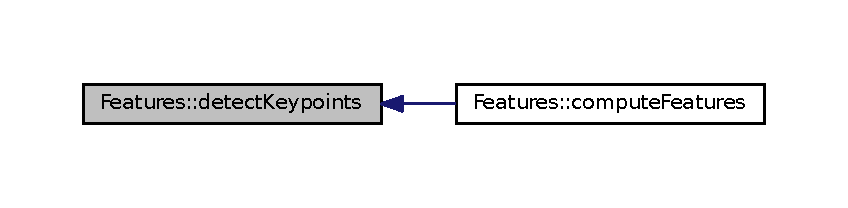
\includegraphics[width=350pt]{class_features_a5c6f5430e675a9216da80875e700f32e_icgraph}
\end{center}
\end{figure}
\hypertarget{class_features_a925cf73afb0607d0fe74a47347ec670d}{}\label{class_features_a925cf73afb0607d0fe74a47347ec670d} 
\index{Features@{Features}!estimate\+Surface\+Normals@{estimate\+Surface\+Normals}}
\index{estimate\+Surface\+Normals@{estimate\+Surface\+Normals}!Features@{Features}}
\subsubsection{\texorpdfstring{estimate\+Surface\+Normals()}{estimateSurfaceNormals()}}
{\footnotesize\ttfamily pcl\+::\+Point\+Cloud$<$ pcl\+::\+Normal $>$\+::Ptr Features\+::estimate\+Surface\+Normals (\begin{DoxyParamCaption}\item[{const pcl\+::\+Point\+Cloud$<$ pcl\+::\+Point\+X\+Y\+Z\+R\+GB $>$\+::Ptr \&}]{input\+Cloud,  }\item[{float}]{radius }\end{DoxyParamCaption})}

Use Normal\+Estimation to estimate a cloud\textquotesingle{}s surface normals Inputs\+: input The input point cloud radius The size of the local neighborhood used to estimate the surface Return\+: A pointer to a Surface\+Normals point cloud 

Definition at line 17 of file features.\+cpp.

Here is the caller graph for this function\+:
\nopagebreak
\begin{figure}[H]
\begin{center}
\leavevmode
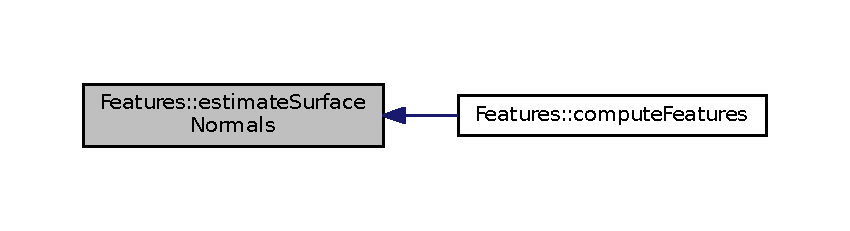
\includegraphics[width=350pt]{class_features_a925cf73afb0607d0fe74a47347ec670d_icgraph}
\end{center}
\end{figure}


The documentation for this class was generated from the following files\+:\begin{DoxyCompactItemize}
\item 
include/\hyperlink{features_8hpp}{features.\+hpp}\item 
src/\hyperlink{features_8cpp}{features.\+cpp}\end{DoxyCompactItemize}

\hypertarget{class_filters}{}\section{Filters Class Reference}
\label{class_filters}\index{Filters@{Filters}}


{\ttfamily \#include $<$filters.\+hpp$>$}

\subsection*{Public Member Functions}
\begin{DoxyCompactItemize}
\item 
pcl\+::\+Point\+Cloud$<$ pcl\+::\+Point\+X\+Y\+Z\+R\+GB $>$\+::Ptr \hyperlink{class_filters_afc0f89a25b158ea0c11025f60fbd9afb}{threshold\+Depth} (const pcl\+::\+Point\+Cloud$<$ pcl\+::\+Point\+X\+Y\+Z\+R\+GB $>$\+::Ptr \&input, float min\+\_\+depth, float max\+\_\+depth)
\item 
pcl\+::\+Point\+Cloud$<$ pcl\+::\+Point\+X\+Y\+Z\+R\+GB $>$\+::Ptr \hyperlink{class_filters_a0435083e1ecca7c1a3d8883f241c4225}{voxelize} (const pcl\+::\+Point\+Cloud$<$ pcl\+::\+Point\+X\+Y\+Z\+R\+GB $>$\+::Ptr \&input, float leaf\+\_\+size)
\item 
pcl\+::\+Point\+Cloud$<$ pcl\+::\+Point\+X\+Y\+Z\+R\+GB $>$\+::Ptr \hyperlink{class_filters_aade8ae78e3f5490db23213b8fc63215b}{remove\+Outliers} (const pcl\+::\+Point\+Cloud$<$ pcl\+::\+Point\+X\+Y\+Z\+R\+GB $>$\+::Ptr \&input, float radius, int min\+\_\+neighbors)
\item 
pcl\+::\+Point\+Cloud$<$ pcl\+::\+Point\+X\+Y\+Z\+R\+GB $>$\+::Ptr \hyperlink{class_filters_a05f3f0a4f537fe94b8f06b9b8b94d48d}{apply\+Filters} (const pcl\+::\+Point\+Cloud$<$ pcl\+::\+Point\+X\+Y\+Z\+R\+GB $>$\+::Ptr \&input, float min\+\_\+depth, float max\+\_\+depth, float leaf\+\_\+size, float radius, float min\+\_\+neighbors)
\item 
pcl\+::\+Point\+Cloud$<$ pcl\+::\+Point\+X\+Y\+Z\+R\+GB $>$\+::Ptr \hyperlink{class_filters_a478cc3062b2a6fff3c2430cb10c86aba}{remove\+Na\+N\+Points} (const pcl\+::\+Point\+Cloud$<$ pcl\+::\+Point\+X\+Y\+Z\+R\+GB $>$\+::Ptr \&input\+Cloud, const std\+::string filename)
\item 
pcl\+::\+Point\+Cloud$<$ pcl\+::\+Point\+Normal $>$\+::Ptr \hyperlink{class_filters_a67a7521cd9568277a9285f214e282a7f}{remove\+Na\+N\+Normals} (const pcl\+::\+Point\+Cloud$<$ pcl\+::\+Point\+Normal $>$\+::Ptr \&input\+Normal, const std\+::string filename)
\end{DoxyCompactItemize}


\subsection{Detailed Description}
This class includes various methods for filtering the point cloud such as reducing number of points in cloud (voxelgrid...) 

Definition at line 11 of file filters.\+hpp.



\subsection{Member Function Documentation}
\hypertarget{class_filters_a05f3f0a4f537fe94b8f06b9b8b94d48d}{}\label{class_filters_a05f3f0a4f537fe94b8f06b9b8b94d48d} 
\index{Filters@{Filters}!apply\+Filters@{apply\+Filters}}
\index{apply\+Filters@{apply\+Filters}!Filters@{Filters}}
\subsubsection{\texorpdfstring{apply\+Filters()}{applyFilters()}}
{\footnotesize\ttfamily pcl\+::\+Point\+Cloud$<$ pcl\+::\+Point\+X\+Y\+Z\+R\+GB $>$\+::Ptr Filters\+::apply\+Filters (\begin{DoxyParamCaption}\item[{const pcl\+::\+Point\+Cloud$<$ pcl\+::\+Point\+X\+Y\+Z\+R\+GB $>$\+::Ptr \&}]{input,  }\item[{float}]{min\+\_\+depth,  }\item[{float}]{max\+\_\+depth,  }\item[{float}]{leaf\+\_\+size,  }\item[{float}]{radius,  }\item[{float}]{min\+\_\+neighbors }\end{DoxyParamCaption})}

Apply a series of filters (threshold depth, downsample, and remove outliers) 

Definition at line 73 of file filters.\+cpp.

Here is the call graph for this function\+:
\nopagebreak
\begin{figure}[H]
\begin{center}
\leavevmode
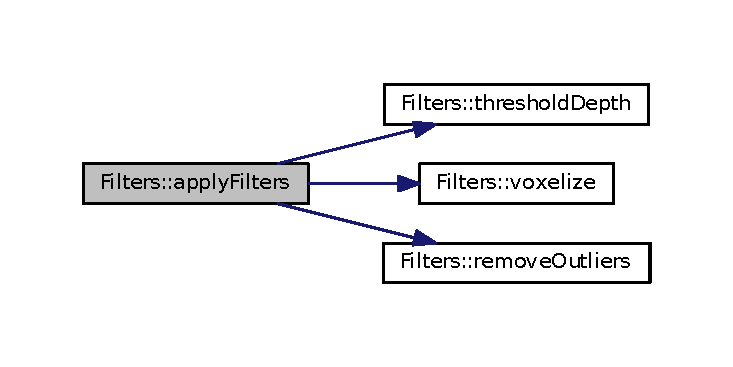
\includegraphics[width=350pt]{class_filters_a05f3f0a4f537fe94b8f06b9b8b94d48d_cgraph}
\end{center}
\end{figure}
\hypertarget{class_filters_a67a7521cd9568277a9285f214e282a7f}{}\label{class_filters_a67a7521cd9568277a9285f214e282a7f} 
\index{Filters@{Filters}!remove\+Na\+N\+Normals@{remove\+Na\+N\+Normals}}
\index{remove\+Na\+N\+Normals@{remove\+Na\+N\+Normals}!Filters@{Filters}}
\subsubsection{\texorpdfstring{remove\+Na\+N\+Normals()}{removeNaNNormals()}}
{\footnotesize\ttfamily pcl\+::\+Point\+Cloud$<$ pcl\+::\+Point\+Normal $>$\+::Ptr Filters\+::remove\+Na\+N\+Normals (\begin{DoxyParamCaption}\item[{const pcl\+::\+Point\+Cloud$<$ pcl\+::\+Point\+Normal $>$\+::Ptr \&}]{input\+Normal,  }\item[{const std\+::string}]{filename }\end{DoxyParamCaption})}

remove all NaN values from Normals 

Definition at line 121 of file filters.\+cpp.

\hypertarget{class_filters_a478cc3062b2a6fff3c2430cb10c86aba}{}\label{class_filters_a478cc3062b2a6fff3c2430cb10c86aba} 
\index{Filters@{Filters}!remove\+Na\+N\+Points@{remove\+Na\+N\+Points}}
\index{remove\+Na\+N\+Points@{remove\+Na\+N\+Points}!Filters@{Filters}}
\subsubsection{\texorpdfstring{remove\+Na\+N\+Points()}{removeNaNPoints()}}
{\footnotesize\ttfamily pcl\+::\+Point\+Cloud$<$ pcl\+::\+Point\+X\+Y\+Z\+R\+GB $>$\+::Ptr Filters\+::remove\+Na\+N\+Points (\begin{DoxyParamCaption}\item[{const pcl\+::\+Point\+Cloud$<$ pcl\+::\+Point\+X\+Y\+Z\+R\+GB $>$\+::Ptr \&}]{input\+Cloud,  }\item[{const std\+::string}]{filename }\end{DoxyParamCaption})}

remove all NaN point cloud values 

Definition at line 89 of file filters.\+cpp.

\hypertarget{class_filters_aade8ae78e3f5490db23213b8fc63215b}{}\label{class_filters_aade8ae78e3f5490db23213b8fc63215b} 
\index{Filters@{Filters}!remove\+Outliers@{remove\+Outliers}}
\index{remove\+Outliers@{remove\+Outliers}!Filters@{Filters}}
\subsubsection{\texorpdfstring{remove\+Outliers()}{removeOutliers()}}
{\footnotesize\ttfamily pcl\+::\+Point\+Cloud$<$ pcl\+::\+Point\+X\+Y\+Z\+R\+GB $>$\+::Ptr Filters\+::remove\+Outliers (\begin{DoxyParamCaption}\item[{const pcl\+::\+Point\+Cloud$<$ pcl\+::\+Point\+X\+Y\+Z\+R\+GB $>$\+::Ptr \&}]{input,  }\item[{float}]{radius,  }\item[{int}]{min\+\_\+neighbors }\end{DoxyParamCaption})}

Use a Radius\+Outlier\+Removal filter to remove all points with too few local neighbors 

Definition at line 55 of file filters.\+cpp.

Here is the caller graph for this function\+:
\nopagebreak
\begin{figure}[H]
\begin{center}
\leavevmode
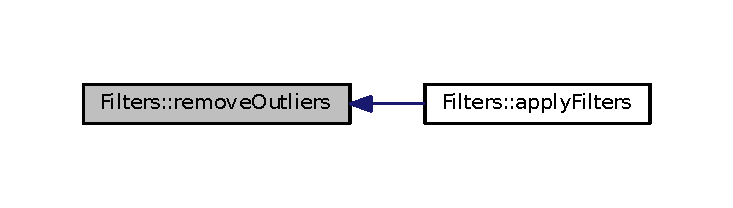
\includegraphics[width=350pt]{class_filters_aade8ae78e3f5490db23213b8fc63215b_icgraph}
\end{center}
\end{figure}
\hypertarget{class_filters_afc0f89a25b158ea0c11025f60fbd9afb}{}\label{class_filters_afc0f89a25b158ea0c11025f60fbd9afb} 
\index{Filters@{Filters}!threshold\+Depth@{threshold\+Depth}}
\index{threshold\+Depth@{threshold\+Depth}!Filters@{Filters}}
\subsubsection{\texorpdfstring{threshold\+Depth()}{thresholdDepth()}}
{\footnotesize\ttfamily pcl\+::\+Point\+Cloud$<$ pcl\+::\+Point\+X\+Y\+Z\+R\+GB $>$\+::Ptr Filters\+::threshold\+Depth (\begin{DoxyParamCaption}\item[{const pcl\+::\+Point\+Cloud$<$ pcl\+::\+Point\+X\+Y\+Z\+R\+GB $>$\+::Ptr \&}]{input,  }\item[{float}]{min\+\_\+depth,  }\item[{float}]{max\+\_\+depth }\end{DoxyParamCaption})}

Use a Pass\+Through filter to remove points with depth values that are too large or too small 

Definition at line 16 of file filters.\+cpp.

Here is the caller graph for this function\+:
\nopagebreak
\begin{figure}[H]
\begin{center}
\leavevmode
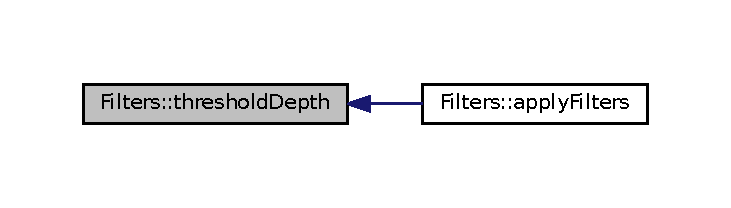
\includegraphics[width=350pt]{class_filters_afc0f89a25b158ea0c11025f60fbd9afb_icgraph}
\end{center}
\end{figure}
\hypertarget{class_filters_a0435083e1ecca7c1a3d8883f241c4225}{}\label{class_filters_a0435083e1ecca7c1a3d8883f241c4225} 
\index{Filters@{Filters}!voxelize@{voxelize}}
\index{voxelize@{voxelize}!Filters@{Filters}}
\subsubsection{\texorpdfstring{voxelize()}{voxelize()}}
{\footnotesize\ttfamily pcl\+::\+Point\+Cloud$<$ pcl\+::\+Point\+X\+Y\+Z\+R\+GB $>$\+::Ptr Filters\+::voxelize (\begin{DoxyParamCaption}\item[{const pcl\+::\+Point\+Cloud$<$ pcl\+::\+Point\+X\+Y\+Z\+R\+GB $>$\+::Ptr \&}]{input,  }\item[{float}]{leaf\+\_\+size }\end{DoxyParamCaption})}

Use a Voxel\+Grid filter to reduce the number of points 

Definition at line 38 of file filters.\+cpp.

Here is the caller graph for this function\+:
\nopagebreak
\begin{figure}[H]
\begin{center}
\leavevmode
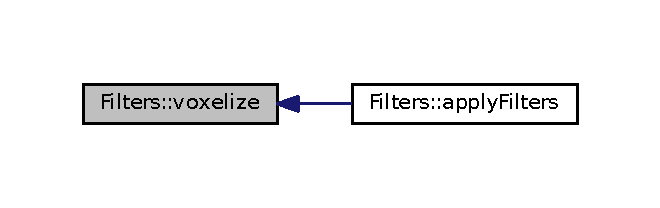
\includegraphics[width=317pt]{class_filters_a0435083e1ecca7c1a3d8883f241c4225_icgraph}
\end{center}
\end{figure}


The documentation for this class was generated from the following files\+:\begin{DoxyCompactItemize}
\item 
include/\hyperlink{filters_8hpp}{filters.\+hpp}\item 
src/\hyperlink{filters_8cpp}{filters.\+cpp}\end{DoxyCompactItemize}

\hypertarget{class_loader}{}\section{Loader Class Reference}
\label{class_loader}\index{Loader@{Loader}}


{\ttfamily \#include $<$loader.\+hpp$>$}

\subsection*{Public Member Functions}
\begin{DoxyCompactItemize}
\item 
boost\+::shared\+\_\+ptr$<$ pcl\+::\+Point\+Cloud$<$ pcl\+::\+Point\+X\+Y\+Z\+R\+GB $>$ $>$ \hyperlink{class_loader_a4a51dc0120d524c010fa2d61c96ffda0}{load\+Point\+Cloud} (std\+::string filename, std\+::string suffix)
\item 
pcl\+::\+Point\+Cloud$<$ pcl\+::\+Point\+X\+Y\+Z\+R\+GB $>$\+::Ptr \hyperlink{class_loader_ae74793144de5bbc0148c257b1f83e0eb}{load\+Points} (std\+::string filename)
\item 
pcl\+::\+Point\+Cloud$<$ pcl\+::\+Normal $>$\+::Ptr \hyperlink{class_loader_a13951e27d82737d95c9ad7b67146f433}{load\+Surface\+Normals} (std\+::string filename)
\item 
pcl\+::\+Point\+Cloud$<$ pcl\+::\+Point\+X\+Y\+Z\+R\+GB $>$\+::Ptr \hyperlink{class_loader_a8cddb9239ed991e33efab83edd7280f7}{load\+Keypoints} (std\+::string filename)
\item 
pcl\+::\+Point\+Cloud$<$ pcl\+::\+F\+P\+F\+H\+Signature33 $>$\+::Ptr \hyperlink{class_loader_ac8938fa9e01e40c2ff21574df60b003a}{load\+Local\+Descriptors} (std\+::string filename)
\item 
pcl\+::\+Point\+Cloud$<$ pcl\+::\+V\+F\+H\+Signature308 $>$\+::Ptr \hyperlink{class_loader_acb76649e253a06ab8c5a475d3fbc74a3}{load\+Global\+Descriptors} (std\+::string filename)
\item 
int \hyperlink{class_loader_ac515e4a910ff4db1e3c1173793bb1bba}{get\+Size} ()
\end{DoxyCompactItemize}


\subsection{Detailed Description}
convenient helper class to load the point clouds from disk 

Definition at line 14 of file loader.\+hpp.



\subsection{Member Function Documentation}
\hypertarget{class_loader_ac515e4a910ff4db1e3c1173793bb1bba}{}\label{class_loader_ac515e4a910ff4db1e3c1173793bb1bba} 
\index{Loader@{Loader}!get\+Size@{get\+Size}}
\index{get\+Size@{get\+Size}!Loader@{Loader}}
\subsubsection{\texorpdfstring{get\+Size()}{getSize()}}
{\footnotesize\ttfamily int Loader\+::get\+Size (\begin{DoxyParamCaption}{ }\end{DoxyParamCaption})}



Definition at line 95 of file loader.\+cpp.

\hypertarget{class_loader_acb76649e253a06ab8c5a475d3fbc74a3}{}\label{class_loader_acb76649e253a06ab8c5a475d3fbc74a3} 
\index{Loader@{Loader}!load\+Global\+Descriptors@{load\+Global\+Descriptors}}
\index{load\+Global\+Descriptors@{load\+Global\+Descriptors}!Loader@{Loader}}
\subsubsection{\texorpdfstring{load\+Global\+Descriptors()}{loadGlobalDescriptors()}}
{\footnotesize\ttfamily pcl\+::\+Point\+Cloud$<$ pcl\+::\+V\+F\+H\+Signature308 $>$\+::Ptr Loader\+::load\+Global\+Descriptors (\begin{DoxyParamCaption}\item[{std\+::string}]{filename }\end{DoxyParamCaption})}



Definition at line 54 of file loader.\+cpp.

\hypertarget{class_loader_a8cddb9239ed991e33efab83edd7280f7}{}\label{class_loader_a8cddb9239ed991e33efab83edd7280f7} 
\index{Loader@{Loader}!load\+Keypoints@{load\+Keypoints}}
\index{load\+Keypoints@{load\+Keypoints}!Loader@{Loader}}
\subsubsection{\texorpdfstring{load\+Keypoints()}{loadKeypoints()}}
{\footnotesize\ttfamily pcl\+::\+Point\+Cloud$<$ pcl\+::\+Point\+X\+Y\+Z\+R\+GB $>$\+::Ptr Loader\+::load\+Keypoints (\begin{DoxyParamCaption}\item[{std\+::string}]{filename }\end{DoxyParamCaption})}



Definition at line 82 of file loader.\+cpp.

\hypertarget{class_loader_ac8938fa9e01e40c2ff21574df60b003a}{}\label{class_loader_ac8938fa9e01e40c2ff21574df60b003a} 
\index{Loader@{Loader}!load\+Local\+Descriptors@{load\+Local\+Descriptors}}
\index{load\+Local\+Descriptors@{load\+Local\+Descriptors}!Loader@{Loader}}
\subsubsection{\texorpdfstring{load\+Local\+Descriptors()}{loadLocalDescriptors()}}
{\footnotesize\ttfamily pcl\+::\+Point\+Cloud$<$ pcl\+::\+F\+P\+F\+H\+Signature33 $>$\+::Ptr Loader\+::load\+Local\+Descriptors (\begin{DoxyParamCaption}\item[{std\+::string}]{filename }\end{DoxyParamCaption})}



Definition at line 40 of file loader.\+cpp.

\hypertarget{class_loader_a4a51dc0120d524c010fa2d61c96ffda0}{}\label{class_loader_a4a51dc0120d524c010fa2d61c96ffda0} 
\index{Loader@{Loader}!load\+Point\+Cloud@{load\+Point\+Cloud}}
\index{load\+Point\+Cloud@{load\+Point\+Cloud}!Loader@{Loader}}
\subsubsection{\texorpdfstring{load\+Point\+Cloud()}{loadPointCloud()}}
{\footnotesize\ttfamily boost\+::shared\+\_\+ptr$<$ pcl\+::\+Point\+Cloud$<$ pcl\+::\+Point\+X\+Y\+Z\+R\+GB $>$ $>$ Loader\+::load\+Point\+Cloud (\begin{DoxyParamCaption}\item[{std\+::string}]{filename,  }\item[{std\+::string}]{suffix }\end{DoxyParamCaption})}



Definition at line 8 of file loader.\+cpp.

\hypertarget{class_loader_ae74793144de5bbc0148c257b1f83e0eb}{}\label{class_loader_ae74793144de5bbc0148c257b1f83e0eb} 
\index{Loader@{Loader}!load\+Points@{load\+Points}}
\index{load\+Points@{load\+Points}!Loader@{Loader}}
\subsubsection{\texorpdfstring{load\+Points()}{loadPoints()}}
{\footnotesize\ttfamily pcl\+::\+Point\+Cloud$<$ pcl\+::\+Point\+X\+Y\+Z\+R\+GB $>$\+::Ptr Loader\+::load\+Points (\begin{DoxyParamCaption}\item[{std\+::string}]{filename }\end{DoxyParamCaption})}



Definition at line 22 of file loader.\+cpp.

\hypertarget{class_loader_a13951e27d82737d95c9ad7b67146f433}{}\label{class_loader_a13951e27d82737d95c9ad7b67146f433} 
\index{Loader@{Loader}!load\+Surface\+Normals@{load\+Surface\+Normals}}
\index{load\+Surface\+Normals@{load\+Surface\+Normals}!Loader@{Loader}}
\subsubsection{\texorpdfstring{load\+Surface\+Normals()}{loadSurfaceNormals()}}
{\footnotesize\ttfamily pcl\+::\+Point\+Cloud$<$ pcl\+::\+Normal $>$\+::Ptr Loader\+::load\+Surface\+Normals (\begin{DoxyParamCaption}\item[{std\+::string}]{filename }\end{DoxyParamCaption})}



Definition at line 68 of file loader.\+cpp.



The documentation for this class was generated from the following files\+:\begin{DoxyCompactItemize}
\item 
include/\hyperlink{loader_8hpp}{loader.\+hpp}\item 
src/\hyperlink{loader_8cpp}{loader.\+cpp}\end{DoxyCompactItemize}

\hypertarget{struct_features_1_1_object_features}{}\section{Features\+:\+:Object\+Features Struct Reference}
\label{struct_features_1_1_object_features}\index{Features\+::\+Object\+Features@{Features\+::\+Object\+Features}}


{\ttfamily \#include $<$features.\+hpp$>$}

\subsection*{Public Attributes}
\begin{DoxyCompactItemize}
\item 
pcl\+::\+Point\+Cloud$<$ pcl\+::\+Point\+X\+Y\+Z\+R\+GB $>$\+::Ptr \hyperlink{struct_features_1_1_object_features_a86f25004593f4c99fd1bbcd3f0d7cf62}{points}
\item 
pcl\+::\+Point\+Cloud$<$ pcl\+::\+Normal $>$\+::Ptr \hyperlink{struct_features_1_1_object_features_ad0d958cfd324196e673ace91e4f57a94}{normals}
\item 
pcl\+::\+Point\+Cloud$<$ pcl\+::\+Point\+X\+Y\+Z\+R\+GB $>$\+::Ptr \hyperlink{struct_features_1_1_object_features_a1d79b5b8a3ed32e75e3bb31bf90e1f27}{keypoints}
\item 
pcl\+::\+Point\+Cloud$<$ pcl\+::\+F\+P\+F\+H\+Signature33 $>$\+::Ptr \hyperlink{struct_features_1_1_object_features_a6a0716472128159b45153c96404ad8c4}{local\+\_\+descriptors}
\item 
pcl\+::\+Point\+Cloud$<$ pcl\+::\+V\+F\+H\+Signature308 $>$\+::Ptr \hyperlink{struct_features_1_1_object_features_a548f1777bc3e5eb3be4c3c3378ac467f}{global\+\_\+descriptor}
\end{DoxyCompactItemize}


\subsection{Detailed Description}
simple structure for storing all of a cloud\textquotesingle{}s features 

Definition at line 17 of file features.\+hpp.



\subsection{Member Data Documentation}
\hypertarget{struct_features_1_1_object_features_a548f1777bc3e5eb3be4c3c3378ac467f}{}\label{struct_features_1_1_object_features_a548f1777bc3e5eb3be4c3c3378ac467f} 
\index{Features\+::\+Object\+Features@{Features\+::\+Object\+Features}!global\+\_\+descriptor@{global\+\_\+descriptor}}
\index{global\+\_\+descriptor@{global\+\_\+descriptor}!Features\+::\+Object\+Features@{Features\+::\+Object\+Features}}
\subsubsection{\texorpdfstring{global\+\_\+descriptor}{global\_descriptor}}
{\footnotesize\ttfamily pcl\+::\+Point\+Cloud$<$pcl\+::\+V\+F\+H\+Signature308$>$\+::Ptr Features\+::\+Object\+Features\+::global\+\_\+descriptor}



Definition at line 22 of file features.\+hpp.

\hypertarget{struct_features_1_1_object_features_a1d79b5b8a3ed32e75e3bb31bf90e1f27}{}\label{struct_features_1_1_object_features_a1d79b5b8a3ed32e75e3bb31bf90e1f27} 
\index{Features\+::\+Object\+Features@{Features\+::\+Object\+Features}!keypoints@{keypoints}}
\index{keypoints@{keypoints}!Features\+::\+Object\+Features@{Features\+::\+Object\+Features}}
\subsubsection{\texorpdfstring{keypoints}{keypoints}}
{\footnotesize\ttfamily pcl\+::\+Point\+Cloud$<$pcl\+::\+Point\+X\+Y\+Z\+R\+GB$>$\+::Ptr Features\+::\+Object\+Features\+::keypoints}



Definition at line 20 of file features.\+hpp.

\hypertarget{struct_features_1_1_object_features_a6a0716472128159b45153c96404ad8c4}{}\label{struct_features_1_1_object_features_a6a0716472128159b45153c96404ad8c4} 
\index{Features\+::\+Object\+Features@{Features\+::\+Object\+Features}!local\+\_\+descriptors@{local\+\_\+descriptors}}
\index{local\+\_\+descriptors@{local\+\_\+descriptors}!Features\+::\+Object\+Features@{Features\+::\+Object\+Features}}
\subsubsection{\texorpdfstring{local\+\_\+descriptors}{local\_descriptors}}
{\footnotesize\ttfamily pcl\+::\+Point\+Cloud$<$pcl\+::\+F\+P\+F\+H\+Signature33$>$\+::Ptr Features\+::\+Object\+Features\+::local\+\_\+descriptors}



Definition at line 21 of file features.\+hpp.

\hypertarget{struct_features_1_1_object_features_ad0d958cfd324196e673ace91e4f57a94}{}\label{struct_features_1_1_object_features_ad0d958cfd324196e673ace91e4f57a94} 
\index{Features\+::\+Object\+Features@{Features\+::\+Object\+Features}!normals@{normals}}
\index{normals@{normals}!Features\+::\+Object\+Features@{Features\+::\+Object\+Features}}
\subsubsection{\texorpdfstring{normals}{normals}}
{\footnotesize\ttfamily pcl\+::\+Point\+Cloud$<$pcl\+::\+Normal$>$\+::Ptr Features\+::\+Object\+Features\+::normals}



Definition at line 19 of file features.\+hpp.

\hypertarget{struct_features_1_1_object_features_a86f25004593f4c99fd1bbcd3f0d7cf62}{}\label{struct_features_1_1_object_features_a86f25004593f4c99fd1bbcd3f0d7cf62} 
\index{Features\+::\+Object\+Features@{Features\+::\+Object\+Features}!points@{points}}
\index{points@{points}!Features\+::\+Object\+Features@{Features\+::\+Object\+Features}}
\subsubsection{\texorpdfstring{points}{points}}
{\footnotesize\ttfamily pcl\+::\+Point\+Cloud$<$pcl\+::\+Point\+X\+Y\+Z\+R\+GB$>$\+::Ptr Features\+::\+Object\+Features\+::points}



Definition at line 18 of file features.\+hpp.



The documentation for this struct was generated from the following file\+:\begin{DoxyCompactItemize}
\item 
include/\hyperlink{features_8hpp}{features.\+hpp}\end{DoxyCompactItemize}

\hypertarget{class_registrator}{}\section{Registrator Class Reference}
\label{class_registrator}\index{Registrator@{Registrator}}


{\ttfamily \#include $<$registrator.\+hpp$>$}

\subsection*{Public Member Functions}
\begin{DoxyCompactItemize}
\item 
Eigen\+::\+Matrix4f \hyperlink{class_registrator_a0430c7ceee244327e61b4c71c0b7c0bd}{compute\+Initial\+Alignment} (const pcl\+::\+Point\+Cloud$<$ pcl\+::\+Point\+X\+Y\+Z\+R\+GB $>$\+::Ptr \&source\+\_\+points, const pcl\+::\+Point\+Cloud$<$ pcl\+::\+F\+P\+F\+H\+Signature33 $>$\+::Ptr \&source\+\_\+descriptors, const pcl\+::\+Point\+Cloud$<$ pcl\+::\+Point\+X\+Y\+Z\+R\+GB $>$\+::Ptr \&target\+\_\+points, const pcl\+::\+Point\+Cloud$<$ pcl\+::\+F\+P\+F\+H\+Signature33 $>$\+::Ptr \&target\+\_\+descriptors, float min\+\_\+sample\+\_\+distance, float max\+\_\+correspondence\+\_\+distance, int nr\+\_\+iterations)
\item 
Eigen\+::\+Matrix4f \hyperlink{class_registrator_af9074af8efbd597162ccfa45b8970656}{refine\+Alignment} (const pcl\+::\+Point\+Cloud$<$ pcl\+::\+Point\+X\+Y\+Z\+R\+GB $>$\+::Ptr \&source\+\_\+points, const pcl\+::\+Point\+Cloud$<$ pcl\+::\+Point\+X\+Y\+Z\+R\+GB $>$\+::Ptr \&target\+\_\+points, const Eigen\+::\+Matrix4f \&initial\+\_\+alignment, float max\+\_\+correspondence\+\_\+distance, float outlier\+\_\+rejection\+\_\+threshold, float transformation\+\_\+epsilon, int max\+\_\+iterations)
\end{DoxyCompactItemize}


\subsection{Detailed Description}
this class computes the initial alignment and refines the alignment using the iterative closest point algorithm 

Definition at line 19 of file registrator.\+hpp.



\subsection{Member Function Documentation}
\hypertarget{class_registrator_a0430c7ceee244327e61b4c71c0b7c0bd}{}\label{class_registrator_a0430c7ceee244327e61b4c71c0b7c0bd} 
\index{Registrator@{Registrator}!compute\+Initial\+Alignment@{compute\+Initial\+Alignment}}
\index{compute\+Initial\+Alignment@{compute\+Initial\+Alignment}!Registrator@{Registrator}}
\subsubsection{\texorpdfstring{compute\+Initial\+Alignment()}{computeInitialAlignment()}}
{\footnotesize\ttfamily Eigen\+::\+Matrix4f Registrator\+::compute\+Initial\+Alignment (\begin{DoxyParamCaption}\item[{const pcl\+::\+Point\+Cloud$<$ pcl\+::\+Point\+X\+Y\+Z\+R\+GB $>$\+::Ptr \&}]{source\+\_\+points,  }\item[{const pcl\+::\+Point\+Cloud$<$ pcl\+::\+F\+P\+F\+H\+Signature33 $>$\+::Ptr \&}]{source\+\_\+descriptors,  }\item[{const pcl\+::\+Point\+Cloud$<$ pcl\+::\+Point\+X\+Y\+Z\+R\+GB $>$\+::Ptr \&}]{target\+\_\+points,  }\item[{const pcl\+::\+Point\+Cloud$<$ pcl\+::\+F\+P\+F\+H\+Signature33 $>$\+::Ptr \&}]{target\+\_\+descriptors,  }\item[{float}]{min\+\_\+sample\+\_\+distance,  }\item[{float}]{max\+\_\+correspondence\+\_\+distance,  }\item[{int}]{nr\+\_\+iterations }\end{DoxyParamCaption})}

Use Sample\+Consensus\+Initial\+Alignment to find a rough alignment from the source cloud to the target cloud by finding correspondences between two sets of local features Inputs\+: source\+\_\+points The \char`\"{}source\char`\"{} points, i.\+e., the points that must be transformed to align with the target point cloud source\+\_\+descriptors The local descriptors for each source point target\+\_\+points The \char`\"{}target\char`\"{} points, i.\+e., the points to which the source point cloud will be aligned target\+\_\+descriptors The local descriptors for each target point min\+\_\+sample\+\_\+distance The minimum distance between any two random samples max\+\_\+correspondence\+\_\+distance The nr\+\_\+interations The number of R\+A\+N\+S\+AC iterations to perform Return\+: A transformation matrix that will roughly align the points in source to the points in target 

Definition at line 62 of file registrator.\+cpp.

\hypertarget{class_registrator_af9074af8efbd597162ccfa45b8970656}{}\label{class_registrator_af9074af8efbd597162ccfa45b8970656} 
\index{Registrator@{Registrator}!refine\+Alignment@{refine\+Alignment}}
\index{refine\+Alignment@{refine\+Alignment}!Registrator@{Registrator}}
\subsubsection{\texorpdfstring{refine\+Alignment()}{refineAlignment()}}
{\footnotesize\ttfamily Eigen\+::\+Matrix4f Registrator\+::refine\+Alignment (\begin{DoxyParamCaption}\item[{const pcl\+::\+Point\+Cloud$<$ pcl\+::\+Point\+X\+Y\+Z\+R\+GB $>$\+::Ptr \&}]{source\+\_\+points,  }\item[{const pcl\+::\+Point\+Cloud$<$ pcl\+::\+Point\+X\+Y\+Z\+R\+GB $>$\+::Ptr \&}]{target\+\_\+points,  }\item[{const Eigen\+::\+Matrix4f \&}]{initial\+\_\+alignment,  }\item[{float}]{max\+\_\+correspondence\+\_\+distance,  }\item[{float}]{outlier\+\_\+rejection\+\_\+threshold,  }\item[{float}]{transformation\+\_\+epsilon,  }\item[{int}]{max\+\_\+iterations }\end{DoxyParamCaption})}

Use Iterative\+Closest\+Point to find a precise alignment from the source cloud to the target cloud, starting with an intial guess Inputs\+: source\+\_\+points The \char`\"{}source\char`\"{} points, i.\+e., the points that must be transformed to align with the target point cloud target\+\_\+points The \char`\"{}target\char`\"{} points, i.\+e., the points to which the source point cloud will be aligned intial\+\_\+alignment An initial estimate of the transformation matrix that aligns the source points to the target points max\+\_\+correspondence\+\_\+distance A threshold on the distance between any two corresponding points. Any corresponding points that are further apart than this threshold will be ignored when computing the source-\/to-\/target transformation outlier\+\_\+rejection\+\_\+threshold A threshold used to define outliers during R\+A\+N\+S\+AC outlier rejection transformation\+\_\+epsilon The smallest iterative transformation allowed before the algorithm is considered to have converged max\+\_\+iterations The maximum number of I\+CP iterations to perform Return\+: A transformation matrix that will precisely align the points in source to the points in target

Use Iterative\+Closest\+Point to find a precise alignment from the source cloud to the target cloud, starting with an initial guess Inputs\+: source\+\_\+points The \char`\"{}source\char`\"{} points, i.\+e., the points that must be transformed to align with the target point cloud target\+\_\+points The \char`\"{}target\char`\"{} points, i.\+e., the points to which the source point cloud will be aligned initial\+\_\+alignment An initial estimate of the transformation matrix that aligns the source points to the target points max\+\_\+correspondence\+\_\+distance A threshold on the distance between any two corresponding points. Any corresponding points that are further apart than this threshold will be ignored when computing the source-\/to-\/target transformation outlier\+\_\+rejection\+\_\+threshold A threshold used to define outliers during R\+A\+N\+S\+AC outlier rejection transformation\+\_\+epsilon The smallest iterative transformation allowed before the algorithm is considered to have converged max\+\_\+iterations The maximum number of I\+CP iterations to perform Return\+: A transformation matrix that will precisely align the points in source to the points in target 

Definition at line 117 of file registrator.\+cpp.



The documentation for this class was generated from the following files\+:\begin{DoxyCompactItemize}
\item 
include/\hyperlink{registrator_8hpp}{registrator.\+hpp}\item 
src/\hyperlink{registrator_8cpp}{registrator.\+cpp}\end{DoxyCompactItemize}

\hypertarget{class_saver}{}\section{Saver Class Reference}
\label{class_saver}\index{Saver@{Saver}}


{\ttfamily \#include $<$loader.\+hpp$>$}

\subsection*{Public Member Functions}
\begin{DoxyCompactItemize}
\item 
int \hyperlink{class_saver_a9d4eb8f7475a1392995cdb24d5b1df12}{save\+Object\+Features} (std\+::string filename, boost\+::shared\+\_\+ptr$<$ \hyperlink{struct_features_1_1_object_features}{Features\+::\+Object\+Features} $>$ \&obj\+Features)
\item 
int \hyperlink{class_saver_a7cb13afc54e63deccb5592a9cafcf023}{save\+Points} (std\+::string filename, pcl\+::\+Point\+Cloud$<$ pcl\+::\+Point\+X\+Y\+Z\+R\+GB $>$\+::Ptr \&points)
\item 
int \hyperlink{class_saver_ae495a4a2592cd981a4085b35f9645d32}{save\+Surface\+Normals} (std\+::string filename, pcl\+::\+Point\+Cloud$<$ pcl\+::\+Normal $>$\+::Ptr \&normals)
\item 
int \hyperlink{class_saver_a11cd83568c660254febecb5cdbeca9e6}{save\+Keypoints} (std\+::string filename, pcl\+::\+Point\+Cloud$<$ pcl\+::\+Point\+X\+Y\+Z\+R\+GB $>$\+::Ptr \&keypoints)
\item 
int \hyperlink{class_saver_a40c302f75d3721d2861a8e93685415ce}{save\+Local\+Descriptors} (std\+::string filename, pcl\+::\+Point\+Cloud$<$ pcl\+::\+F\+P\+F\+H\+Signature33 $>$\+::Ptr \&signature)
\item 
int \hyperlink{class_saver_a19a78a945fdc1da9193d46054a6ad80a}{save\+Global\+Descriptors} (std\+::string filename, pcl\+::\+Point\+Cloud$<$ pcl\+::\+V\+F\+H\+Signature308 $>$\+::Ptr \&signature)
\end{DoxyCompactItemize}


\subsection{Detailed Description}
convenient helper class to save the point clouds to disk 

Definition at line 51 of file loader.\+hpp.



\subsection{Member Function Documentation}
\hypertarget{class_saver_a19a78a945fdc1da9193d46054a6ad80a}{}\label{class_saver_a19a78a945fdc1da9193d46054a6ad80a} 
\index{Saver@{Saver}!save\+Global\+Descriptors@{save\+Global\+Descriptors}}
\index{save\+Global\+Descriptors@{save\+Global\+Descriptors}!Saver@{Saver}}
\subsubsection{\texorpdfstring{save\+Global\+Descriptors()}{saveGlobalDescriptors()}}
{\footnotesize\ttfamily int Saver\+::save\+Global\+Descriptors (\begin{DoxyParamCaption}\item[{std\+::string}]{filename,  }\item[{pcl\+::\+Point\+Cloud$<$ pcl\+::\+V\+F\+H\+Signature308 $>$\+::Ptr \&}]{signature }\end{DoxyParamCaption})}



Definition at line 105 of file loader.\+cpp.

\hypertarget{class_saver_a11cd83568c660254febecb5cdbeca9e6}{}\label{class_saver_a11cd83568c660254febecb5cdbeca9e6} 
\index{Saver@{Saver}!save\+Keypoints@{save\+Keypoints}}
\index{save\+Keypoints@{save\+Keypoints}!Saver@{Saver}}
\subsubsection{\texorpdfstring{save\+Keypoints()}{saveKeypoints()}}
{\footnotesize\ttfamily int Saver\+::save\+Keypoints (\begin{DoxyParamCaption}\item[{std\+::string}]{filename,  }\item[{pcl\+::\+Point\+Cloud$<$ pcl\+::\+Point\+X\+Y\+Z\+R\+GB $>$\+::Ptr \&}]{keypoints }\end{DoxyParamCaption})}



Definition at line 127 of file loader.\+cpp.

\hypertarget{class_saver_a40c302f75d3721d2861a8e93685415ce}{}\label{class_saver_a40c302f75d3721d2861a8e93685415ce} 
\index{Saver@{Saver}!save\+Local\+Descriptors@{save\+Local\+Descriptors}}
\index{save\+Local\+Descriptors@{save\+Local\+Descriptors}!Saver@{Saver}}
\subsubsection{\texorpdfstring{save\+Local\+Descriptors()}{saveLocalDescriptors()}}
{\footnotesize\ttfamily int Saver\+::save\+Local\+Descriptors (\begin{DoxyParamCaption}\item[{std\+::string}]{filename,  }\item[{pcl\+::\+Point\+Cloud$<$ pcl\+::\+F\+P\+F\+H\+Signature33 $>$\+::Ptr \&}]{signature }\end{DoxyParamCaption})}



Definition at line 116 of file loader.\+cpp.

\hypertarget{class_saver_a9d4eb8f7475a1392995cdb24d5b1df12}{}\label{class_saver_a9d4eb8f7475a1392995cdb24d5b1df12} 
\index{Saver@{Saver}!save\+Object\+Features@{save\+Object\+Features}}
\index{save\+Object\+Features@{save\+Object\+Features}!Saver@{Saver}}
\subsubsection{\texorpdfstring{save\+Object\+Features()}{saveObjectFeatures()}}
{\footnotesize\ttfamily int Saver\+::save\+Object\+Features (\begin{DoxyParamCaption}\item[{std\+::string}]{filename,  }\item[{boost\+::shared\+\_\+ptr$<$ \hyperlink{struct_features_1_1_object_features}{Features\+::\+Object\+Features} $>$ \&}]{obj\+Features }\end{DoxyParamCaption})}



Definition at line 159 of file loader.\+cpp.

\hypertarget{class_saver_a7cb13afc54e63deccb5592a9cafcf023}{}\label{class_saver_a7cb13afc54e63deccb5592a9cafcf023} 
\index{Saver@{Saver}!save\+Points@{save\+Points}}
\index{save\+Points@{save\+Points}!Saver@{Saver}}
\subsubsection{\texorpdfstring{save\+Points()}{savePoints()}}
{\footnotesize\ttfamily int Saver\+::save\+Points (\begin{DoxyParamCaption}\item[{std\+::string}]{filename,  }\item[{pcl\+::\+Point\+Cloud$<$ pcl\+::\+Point\+X\+Y\+Z\+R\+GB $>$\+::Ptr \&}]{points }\end{DoxyParamCaption})}



Definition at line 149 of file loader.\+cpp.

\hypertarget{class_saver_ae495a4a2592cd981a4085b35f9645d32}{}\label{class_saver_ae495a4a2592cd981a4085b35f9645d32} 
\index{Saver@{Saver}!save\+Surface\+Normals@{save\+Surface\+Normals}}
\index{save\+Surface\+Normals@{save\+Surface\+Normals}!Saver@{Saver}}
\subsubsection{\texorpdfstring{save\+Surface\+Normals()}{saveSurfaceNormals()}}
{\footnotesize\ttfamily int Saver\+::save\+Surface\+Normals (\begin{DoxyParamCaption}\item[{std\+::string}]{filename,  }\item[{pcl\+::\+Point\+Cloud$<$ pcl\+::\+Normal $>$\+::Ptr \&}]{normals }\end{DoxyParamCaption})}



Definition at line 138 of file loader.\+cpp.



The documentation for this class was generated from the following files\+:\begin{DoxyCompactItemize}
\item 
include/\hyperlink{loader_8hpp}{loader.\+hpp}\item 
src/\hyperlink{loader_8cpp}{loader.\+cpp}\end{DoxyCompactItemize}

\chapter{File Documentation}
\hypertarget{features_8hpp}{}\section{include/features.hpp File Reference}
\label{features_8hpp}\index{include/features.\+hpp@{include/features.\+hpp}}
{\ttfamily \#include $<$pcl/point\+\_\+types.\+h$>$}\newline
{\ttfamily \#include $<$pcl/point\+\_\+cloud.\+h$>$}\newline
Include dependency graph for features.\+hpp\+:
\nopagebreak
\begin{figure}[H]
\begin{center}
\leavevmode
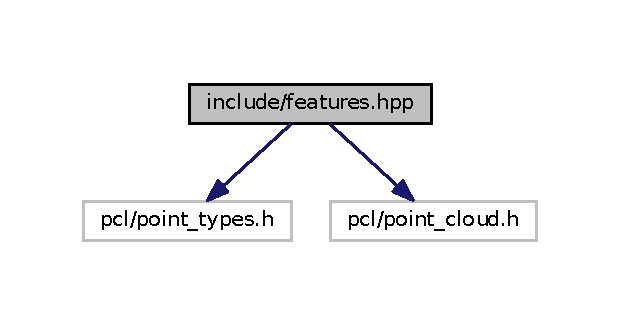
\includegraphics[width=298pt]{features_8hpp__incl}
\end{center}
\end{figure}
This graph shows which files directly or indirectly include this file\+:
\nopagebreak
\begin{figure}[H]
\begin{center}
\leavevmode
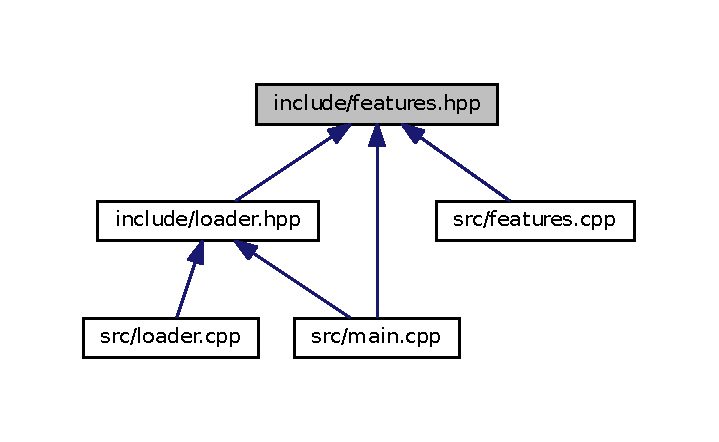
\includegraphics[width=345pt]{features_8hpp__dep__incl}
\end{center}
\end{figure}
\subsection*{Classes}
\begin{DoxyCompactItemize}
\item 
class \hyperlink{class_features}{Features}
\item 
struct \hyperlink{struct_features_1_1_object_features}{Features\+::\+Object\+Features}
\end{DoxyCompactItemize}

\hypertarget{filters_8hpp}{}\section{include/filters.hpp File Reference}
\label{filters_8hpp}\index{include/filters.\+hpp@{include/filters.\+hpp}}
{\ttfamily \#include $<$pcl/point\+\_\+types.\+h$>$}\newline
{\ttfamily \#include $<$pcl/point\+\_\+cloud.\+h$>$}\newline
Include dependency graph for filters.\+hpp\+:
\nopagebreak
\begin{figure}[H]
\begin{center}
\leavevmode
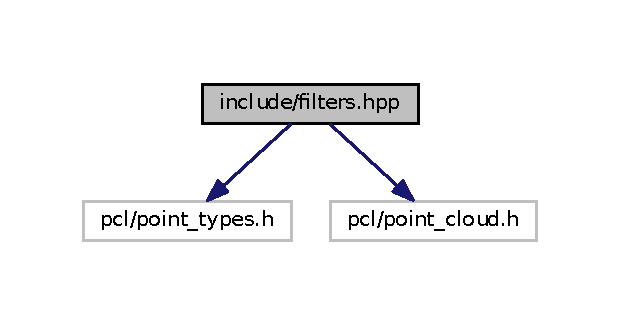
\includegraphics[width=298pt]{filters_8hpp__incl}
\end{center}
\end{figure}
This graph shows which files directly or indirectly include this file\+:
\nopagebreak
\begin{figure}[H]
\begin{center}
\leavevmode
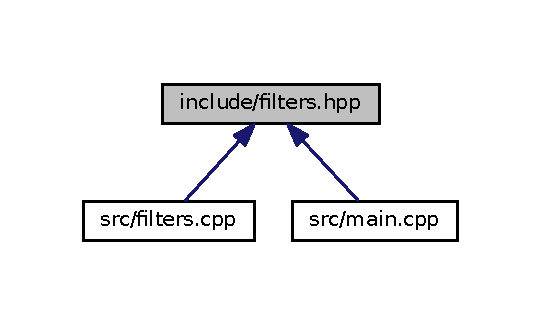
\includegraphics[width=260pt]{filters_8hpp__dep__incl}
\end{center}
\end{figure}
\subsection*{Classes}
\begin{DoxyCompactItemize}
\item 
class \hyperlink{class_filters}{Filters}
\end{DoxyCompactItemize}

\hypertarget{loader_8hpp}{}\section{include/loader.hpp File Reference}
\label{loader_8hpp}\index{include/loader.\+hpp@{include/loader.\+hpp}}
{\ttfamily \#include $<$pcl/point\+\_\+types.\+h$>$}\newline
{\ttfamily \#include $<$pcl/point\+\_\+cloud.\+h$>$}\newline
{\ttfamily \#include $<$string.\+h$>$}\newline
{\ttfamily \#include \char`\"{}features.\+hpp\char`\"{}}\newline
Include dependency graph for loader.\+hpp\+:
\nopagebreak
\begin{figure}[H]
\begin{center}
\leavevmode
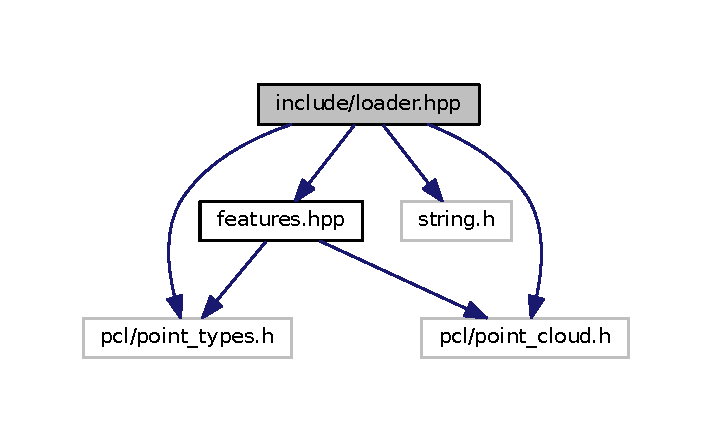
\includegraphics[width=342pt]{loader_8hpp__incl}
\end{center}
\end{figure}
This graph shows which files directly or indirectly include this file\+:
\nopagebreak
\begin{figure}[H]
\begin{center}
\leavevmode
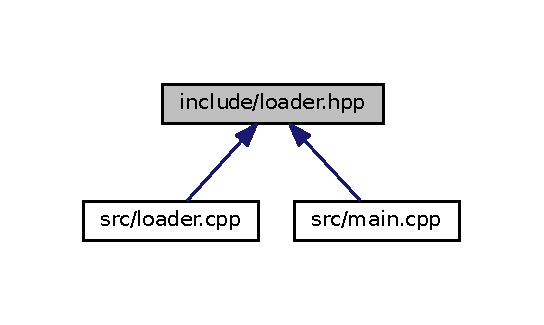
\includegraphics[width=261pt]{loader_8hpp__dep__incl}
\end{center}
\end{figure}
\subsection*{Classes}
\begin{DoxyCompactItemize}
\item 
class \hyperlink{class_loader}{Loader}
\item 
class \hyperlink{class_saver}{Saver}
\end{DoxyCompactItemize}

\hypertarget{registrator_8hpp}{}\section{include/registrator.hpp File Reference}
\label{registrator_8hpp}\index{include/registrator.\+hpp@{include/registrator.\+hpp}}
{\ttfamily \#include $<$string.\+h$>$}\newline
{\ttfamily \#include $<$pcl/point\+\_\+types.\+h$>$}\newline
{\ttfamily \#include $<$pcl/point\+\_\+cloud.\+h$>$}\newline
{\ttfamily \#include $<$pcl/features/fpfh.\+h$>$}\newline
{\ttfamily \#include $<$pcl/features/pfh.\+h$>$}\newline
{\ttfamily \#include $<$Eigen/\+Geometry$>$}\newline
{\ttfamily \#include $<$pcl/keypoints/sift\+\_\+keypoint.\+h$>$}\newline
{\ttfamily \#include $<$pcl/search/impl/search.\+hpp$>$}\newline
Include dependency graph for registrator.\+hpp\+:
\nopagebreak
\begin{figure}[H]
\begin{center}
\leavevmode
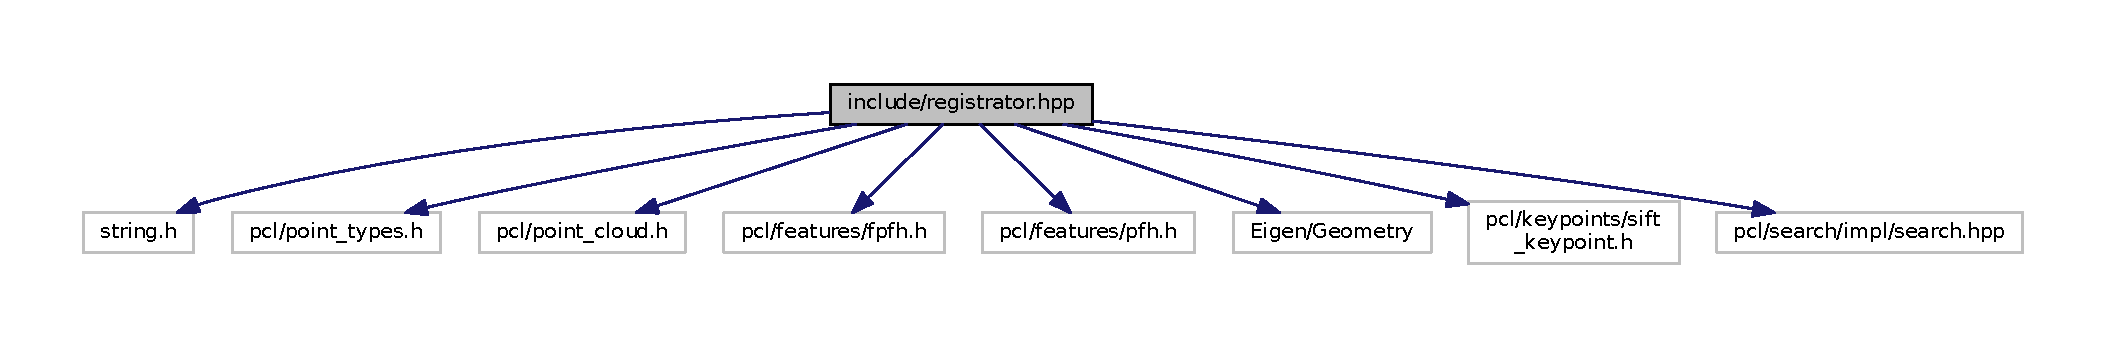
\includegraphics[width=350pt]{registrator_8hpp__incl}
\end{center}
\end{figure}
This graph shows which files directly or indirectly include this file\+:
\nopagebreak
\begin{figure}[H]
\begin{center}
\leavevmode
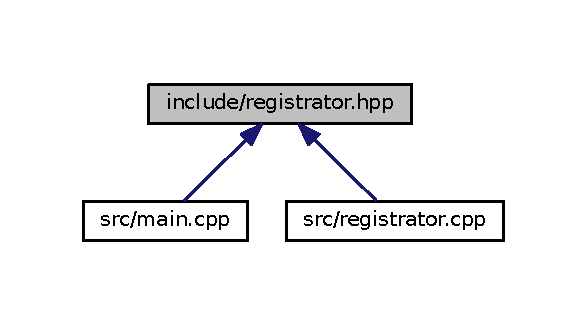
\includegraphics[width=282pt]{registrator_8hpp__dep__incl}
\end{center}
\end{figure}
\subsection*{Classes}
\begin{DoxyCompactItemize}
\item 
class \hyperlink{class_registrator}{Registrator}
\end{DoxyCompactItemize}

\hypertarget{features_8cpp}{}\section{src/features.cpp File Reference}
\label{features_8cpp}\index{src/features.\+cpp@{src/features.\+cpp}}
{\ttfamily \#include \char`\"{}features.\+hpp\char`\"{}}\newline
{\ttfamily \#include $<$pcl/impl/point\+\_\+types.\+hpp$>$}\newline
{\ttfamily \#include $<$pcl/point\+\_\+cloud.\+h$>$}\newline
{\ttfamily \#include $<$pcl/search/kdtree.\+h$>$}\newline
{\ttfamily \#include $<$pcl/keypoints/sift\+\_\+keypoint.\+h$>$}\newline
{\ttfamily \#include $<$pcl/features/normal\+\_\+3d.\+h$>$}\newline
{\ttfamily \#include $<$pcl/features/fpfh.\+h$>$}\newline
{\ttfamily \#include $<$pcl/features/vfh.\+h$>$}\newline
{\ttfamily \#include $<$pcl/search/impl/search.\+hpp$>$}\newline
{\ttfamily \#include $<$boost/shared\+\_\+ptr.\+hpp$>$}\newline
Include dependency graph for features.\+cpp\+:
\nopagebreak
\begin{figure}[H]
\begin{center}
\leavevmode
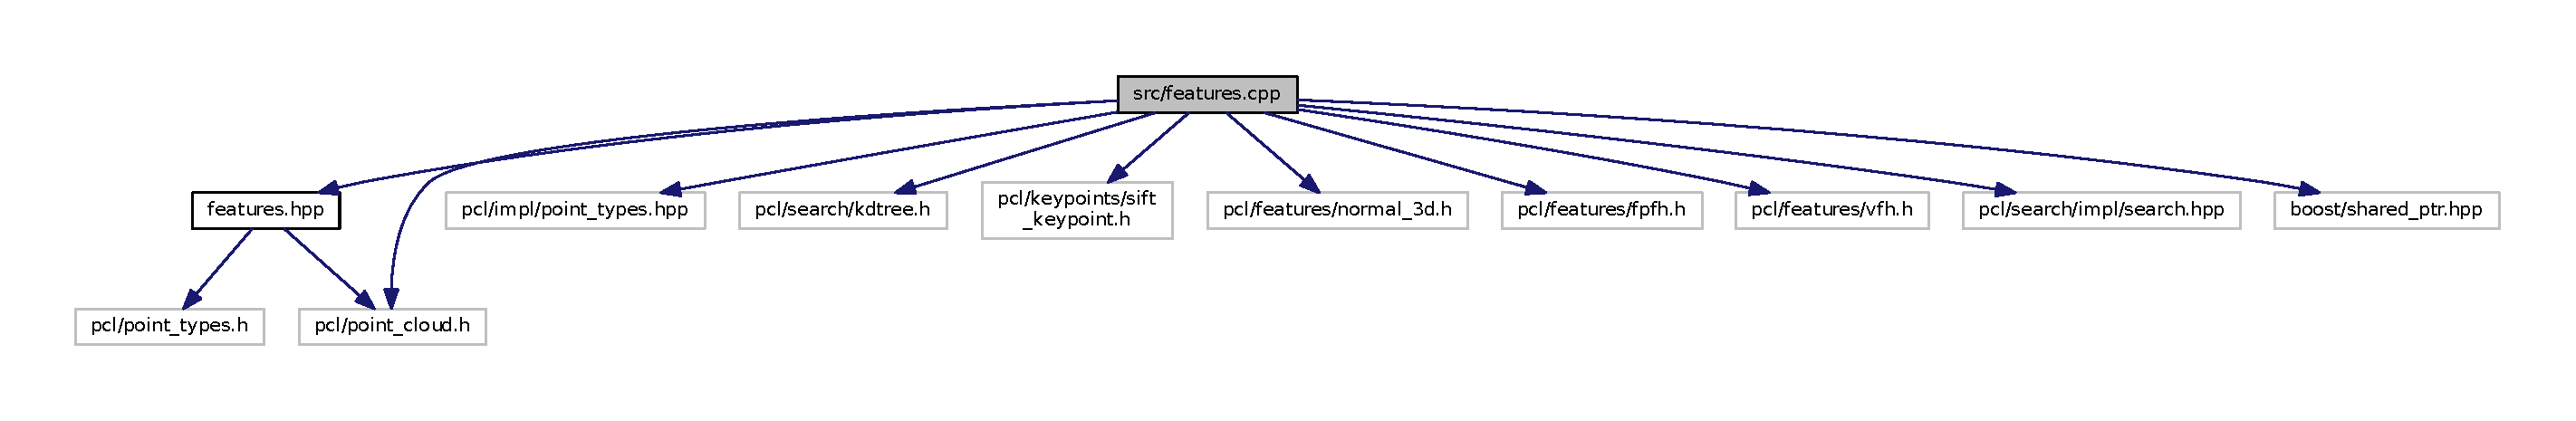
\includegraphics[width=350pt]{features_8cpp__incl}
\end{center}
\end{figure}

\hypertarget{filters_8cpp}{}\section{src/filters.cpp File Reference}
\label{filters_8cpp}\index{src/filters.\+cpp@{src/filters.\+cpp}}
{\ttfamily \#include \char`\"{}filters.\+hpp\char`\"{}}\newline
{\ttfamily \#include $<$pcl/filters/radius\+\_\+outlier\+\_\+removal.\+h$>$}\newline
{\ttfamily \#include $<$pcl/filters/voxel\+\_\+grid.\+h$>$}\newline
{\ttfamily \#include $<$pcl/filters/passthrough.\+h$>$}\newline
{\ttfamily \#include $<$pcl/filters/filter.\+h$>$}\newline
{\ttfamily \#include $<$iostream$>$}\newline
{\ttfamily \#include $<$limits$>$}\newline
Include dependency graph for filters.\+cpp\+:
\nopagebreak
\begin{figure}[H]
\begin{center}
\leavevmode
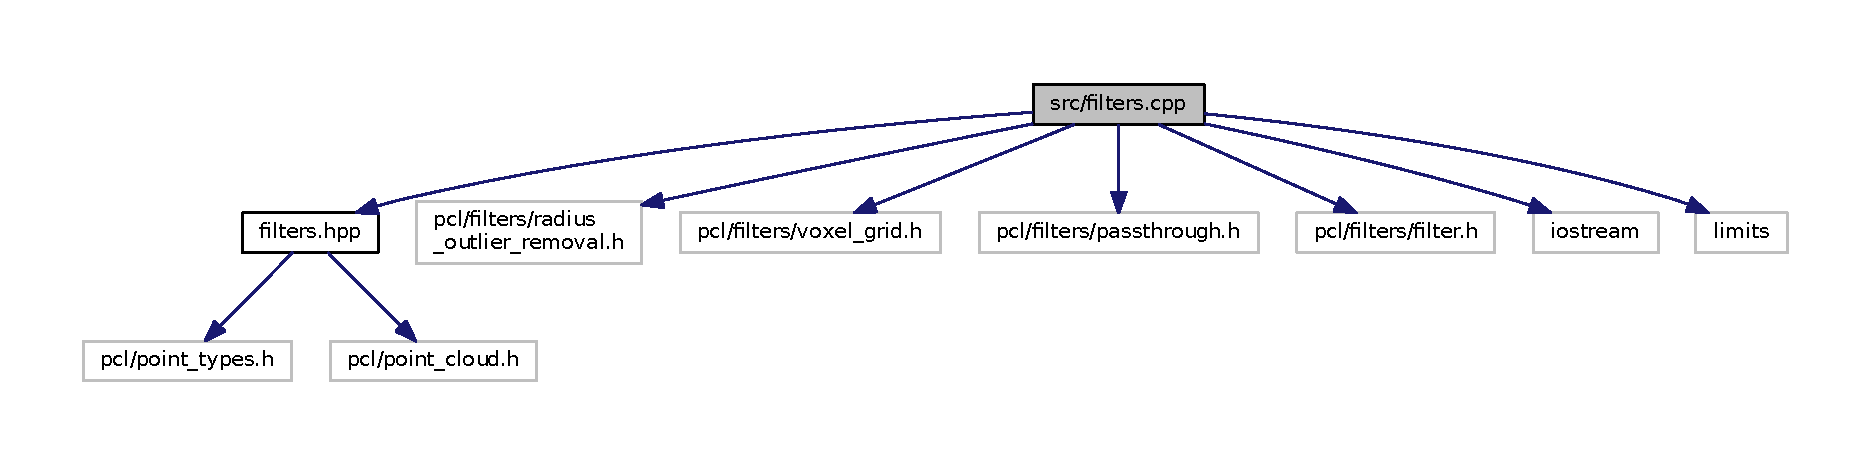
\includegraphics[width=350pt]{filters_8cpp__incl}
\end{center}
\end{figure}

\hypertarget{loader_8cpp}{}\section{src/loader.cpp File Reference}
\label{loader_8cpp}\index{src/loader.\+cpp@{src/loader.\+cpp}}
{\ttfamily \#include \char`\"{}loader.\+hpp\char`\"{}}\newline
{\ttfamily \#include $<$pcl/console/print.\+h$>$}\newline
{\ttfamily \#include $<$pcl/io/pcd\+\_\+io.\+h$>$}\newline
Include dependency graph for loader.\+cpp\+:
\nopagebreak
\begin{figure}[H]
\begin{center}
\leavevmode
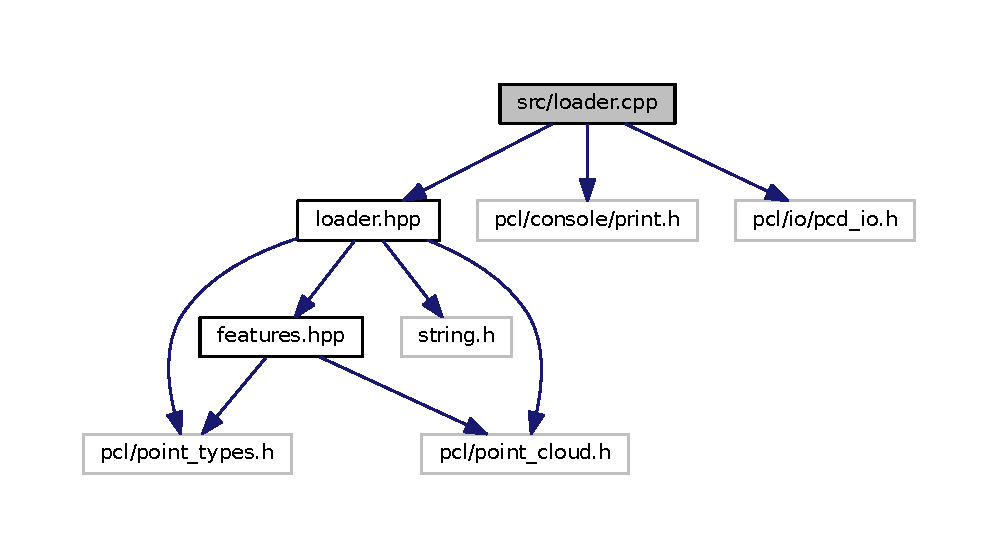
\includegraphics[width=350pt]{loader_8cpp__incl}
\end{center}
\end{figure}

\hypertarget{main_8cpp}{}\section{src/main.cpp File Reference}
\label{main_8cpp}\index{src/main.\+cpp@{src/main.\+cpp}}
{\ttfamily \#include \char`\"{}registrator.\+hpp\char`\"{}}\newline
{\ttfamily \#include \char`\"{}filters.\+hpp\char`\"{}}\newline
{\ttfamily \#include \char`\"{}features.\+hpp\char`\"{}}\newline
{\ttfamily \#include \char`\"{}loader.\+hpp\char`\"{}}\newline
{\ttfamily \#include $<$pcl/io/boost.\+h$>$}\newline
{\ttfamily \#include $<$boost/make\+\_\+shared.\+hpp$>$}\newline
{\ttfamily \#include $<$pcl/common/transforms.\+h$>$}\newline
{\ttfamily \#include $<$pcl/console/parse.\+h$>$}\newline
{\ttfamily \#include $<$pcl/io/pcd\+\_\+io.\+h$>$}\newline
{\ttfamily \#include $<$pcl/visualization/pcl\+\_\+visualizer.\+h$>$}\newline
{\ttfamily \#include $<$boost/program\+\_\+options.\+hpp$>$}\newline
Include dependency graph for main.\+cpp\+:
\nopagebreak
\begin{figure}[H]
\begin{center}
\leavevmode
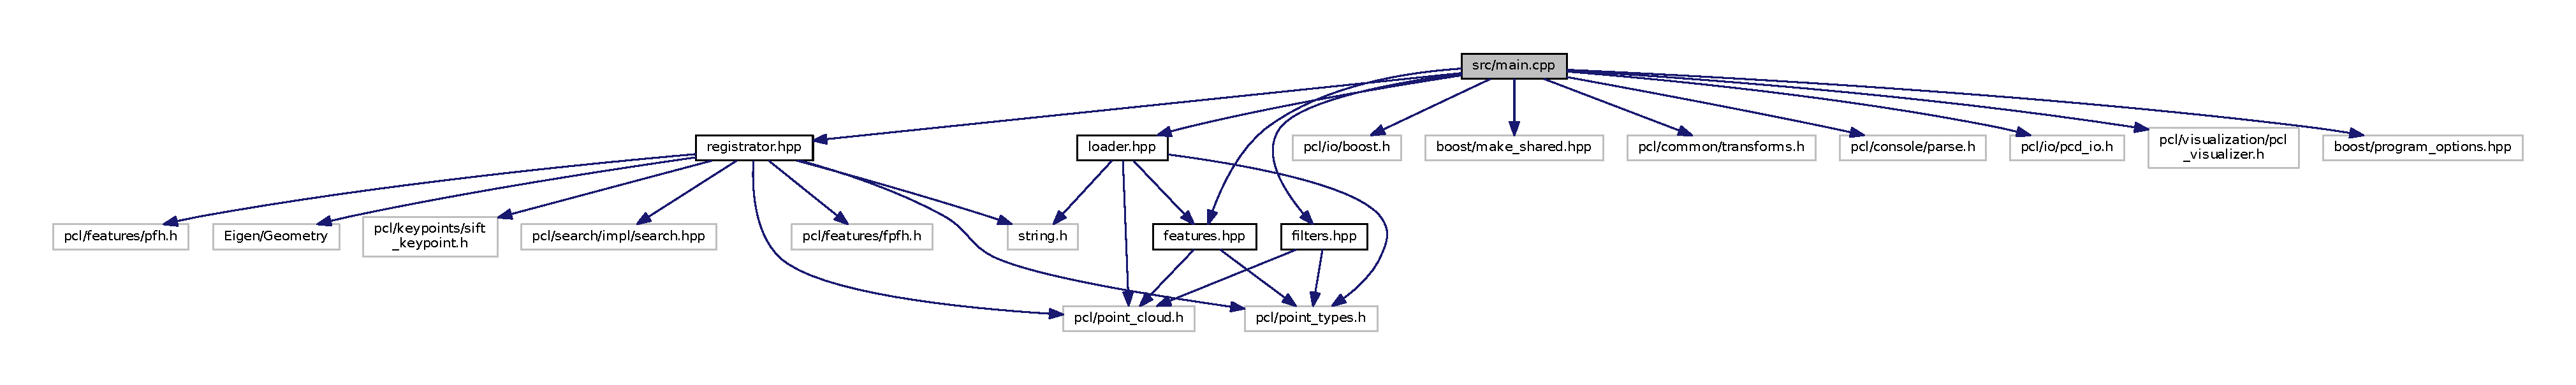
\includegraphics[width=350pt]{main_8cpp__incl}
\end{center}
\end{figure}
\subsection*{Functions}
\begin{DoxyCompactItemize}
\item 
int \hyperlink{main_8cpp_a3c04138a5bfe5d72780bb7e82a18e627}{main} (int argc, char $\ast$$\ast$argv)
\end{DoxyCompactItemize}


\subsection{Function Documentation}
\hypertarget{main_8cpp_a3c04138a5bfe5d72780bb7e82a18e627}{}\label{main_8cpp_a3c04138a5bfe5d72780bb7e82a18e627} 
\index{main.\+cpp@{main.\+cpp}!main@{main}}
\index{main@{main}!main.\+cpp@{main.\+cpp}}
\subsubsection{\texorpdfstring{main()}{main()}}
{\footnotesize\ttfamily int main (\begin{DoxyParamCaption}\item[{int}]{argc,  }\item[{char $\ast$$\ast$}]{argv }\end{DoxyParamCaption})}



Definition at line 20 of file main.\+cpp.


\hypertarget{registrator_8cpp}{}\section{src/registrator.cpp File Reference}
\label{registrator_8cpp}\index{src/registrator.\+cpp@{src/registrator.\+cpp}}
{\ttfamily \#include \char`\"{}registrator.\+hpp\char`\"{}}\newline
{\ttfamily \#include $<$pcl/search/impl/search.\+hpp$>$}\newline
{\ttfamily \#include $<$pcl/registration/icp.\+h$>$}\newline
{\ttfamily \#include $<$pcl/features/normal\+\_\+3d.\+h$>$}\newline
{\ttfamily \#include $<$pcl/filters/radius\+\_\+outlier\+\_\+removal.\+h$>$}\newline
{\ttfamily \#include $<$pcl/search/kdtree.\+h$>$}\newline
{\ttfamily \#include $<$pcl/impl/point\+\_\+types.\+hpp$>$}\newline
{\ttfamily \#include $<$pcl/registration/sample\+\_\+consensus\+\_\+prerejective.\+h$>$}\newline
{\ttfamily \#include $<$pcl/keypoints/harris\+\_\+3d.\+h$>$}\newline
{\ttfamily \#include $<$pcl/features/vfh.\+h$>$}\newline
{\ttfamily \#include $<$pcl/registration/correspondence\+\_\+rejection\+\_\+sample\+\_\+consensus.\+h$>$}\newline
{\ttfamily \#include $<$pcl/filters/approximate\+\_\+voxel\+\_\+grid.\+h$>$}\newline
{\ttfamily \#include $<$pcl/visualization/pcl\+\_\+visualizer.\+h$>$}\newline
{\ttfamily \#include $<$pcl/filters/statistical\+\_\+outlier\+\_\+removal.\+h$>$}\newline
{\ttfamily \#include $<$pcl/io/pcd\+\_\+io.\+h$>$}\newline
{\ttfamily \#include $<$pcl/filters/voxel\+\_\+grid.\+h$>$}\newline
{\ttfamily \#include $<$pcl/registration/ia\+\_\+ransac.\+h$>$}\newline
{\ttfamily \#include $<$pcl/registration/ndt.\+h$>$}\newline
{\ttfamily \#include $<$pcl/registration/icp\+\_\+nl.\+h$>$}\newline
{\ttfamily \#include $<$pcl/keypoints/sift\+\_\+keypoint.\+h$>$}\newline
{\ttfamily \#include $<$pcl/registration/correspondence\+\_\+rejection\+\_\+features.\+h$>$}\newline
{\ttfamily \#include $<$boost/shared\+\_\+ptr.\+hpp$>$}\newline
{\ttfamily \#include $<$boost/make\+\_\+shared.\+hpp$>$}\newline
{\ttfamily \#include $<$string.\+h$>$}\newline
Include dependency graph for registrator.\+cpp\+:
\nopagebreak
\begin{figure}[H]
\begin{center}
\leavevmode
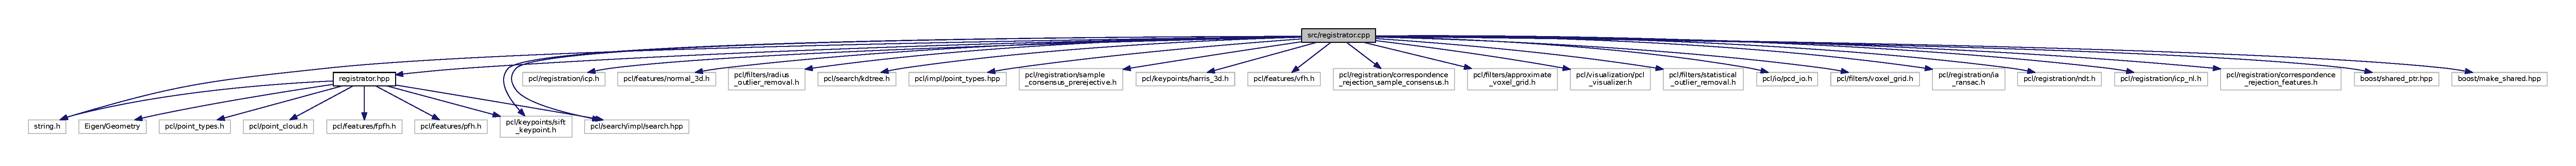
\includegraphics[width=350pt]{registrator_8cpp__incl}
\end{center}
\end{figure}

%--- End generated contents ---

% Index
\backmatter
\newpage
\phantomsection
\clearemptydoublepage
\addcontentsline{toc}{chapter}{Index}
\printindex

\end{document}
